\chapter{Verification Plan}\label{verification}

\section{Verification Plan}

Validation plan and testing is the process of evaluating a system or component during or at the end of the development process to determine whether it satisfies specified requirements.

\begin{enumerate}

\item \textbf{Integration Test:}Integration tests verify that the major software components within the system work correctly with other components within the system, and as specified in the architectural design. Figure 6.1 shows the component packages that form the MASS application. The arrows represent the order of the integration i.e. integration testing. The integration tests of lower level code modules are described in the corresponding component packages unit test. We will provide a detailed test case specification for each module. In order to decide the number of integration tests we consider the following two criteria's:

\subitem 1) Check that all data exchanged across an interface agrees with the data structure specifications.
\subitem 2)Confirm that all the control flows have been implemented.

\begin{figure}[H]
\centering
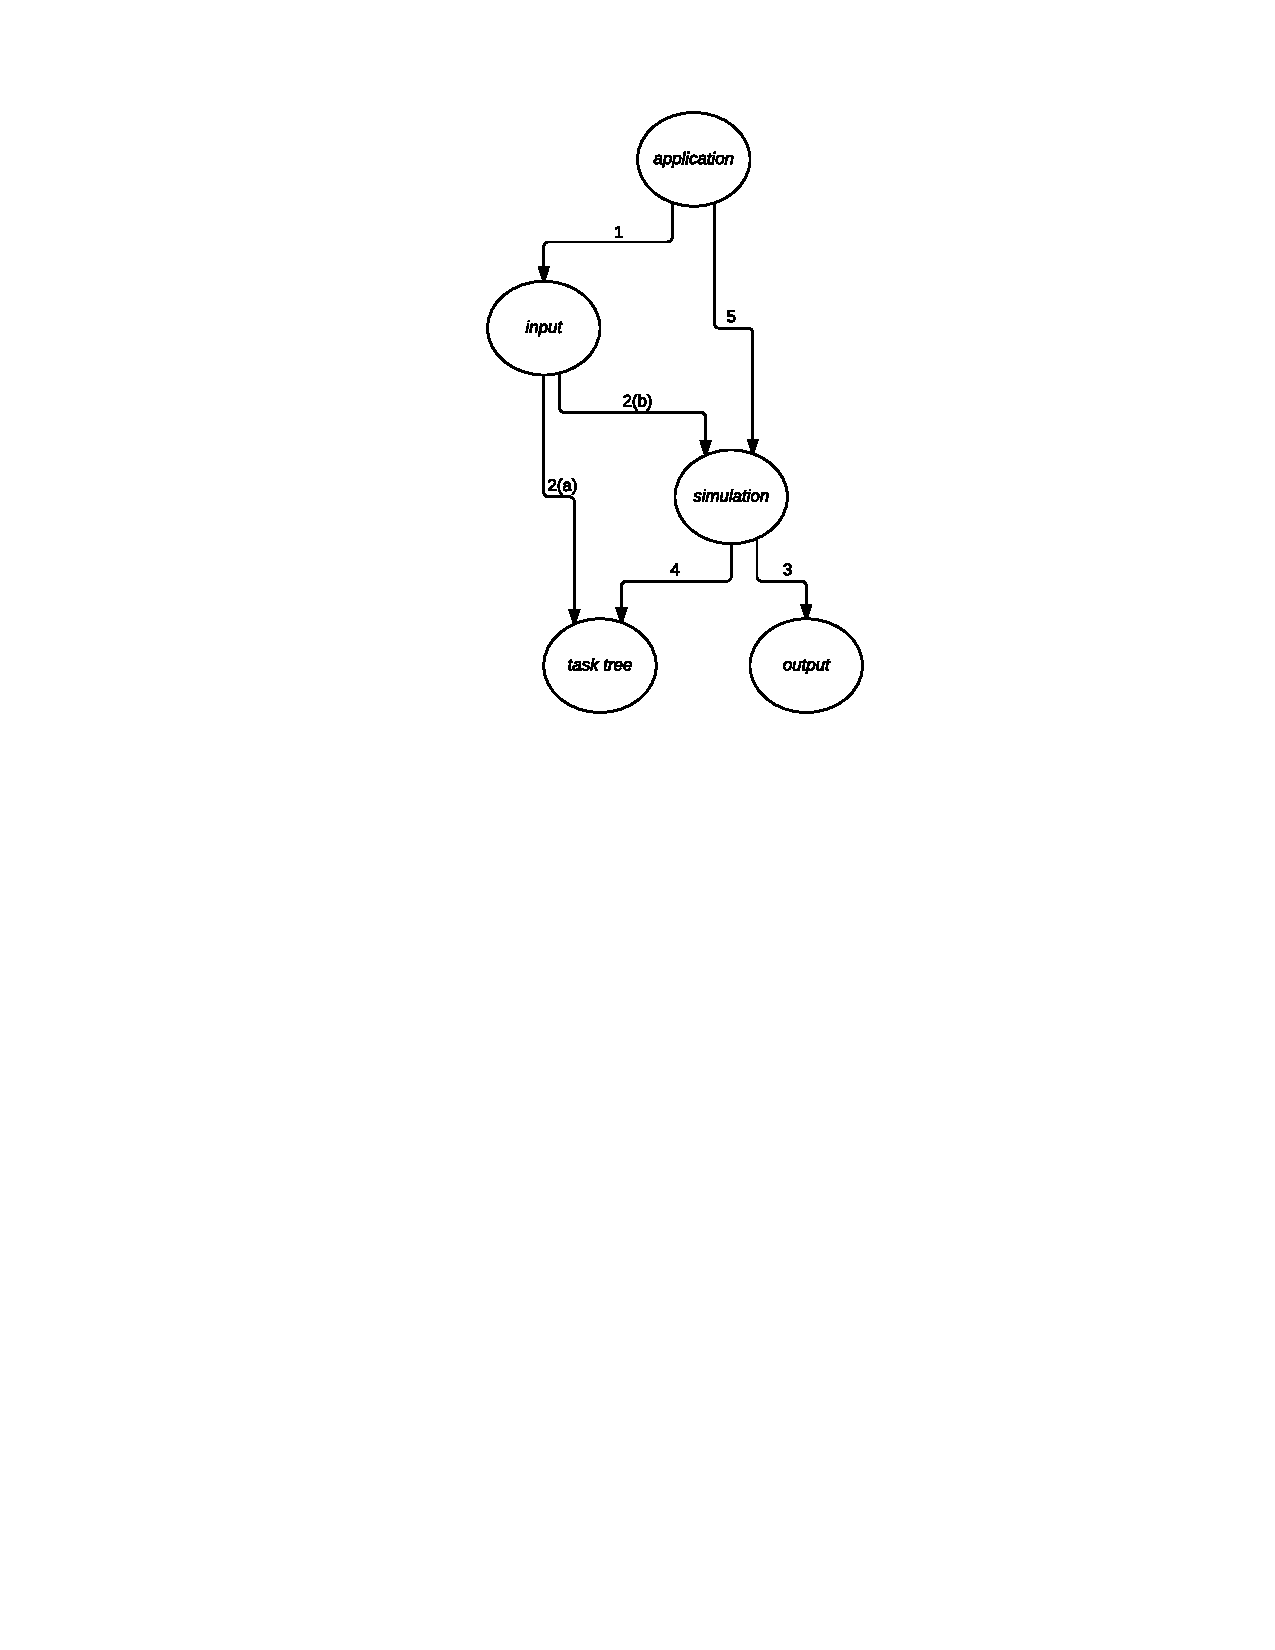
\includegraphics[width=6.0in]{figs/OverviewUsesDiagram}
\caption{Overview of the USES diagram for packages within MASS.}
\label{fig:OverviewUsesDiagram }
\end{figure}

\item \textbf{System Tests:} In order to verify that the software system meets the software requirements we perform system tests.  Wherever possible, system tests should be specified and performed by an independent testing team. This increases the objectivity of the tests and reduces the likelihood of defects escaping the software verification and validation net. Knowledge of the internal workings of the software is not required as a result we use Black-box test method.

\item \textbf{Black box testing:} The objective of black-box testing is to verify the functionality of the Simulator. Here, each module is treated as a `black-box', whose internals cannot be seen. We examine the specification of each module by defining different input scenarios that would result in different behavior.
 
\item \textbf{Input Data:}
 
\item \textbf{Configuration File Input (CFI):} This module accepts a plain text configuration file in the current directory. We classify this input data into a set of equivalence classes.  For any given error, input data sets in the same equivalence class will produce the same error.
 
\item\textbf{Equivalence Classes for Configuration File Input (CFI):}
 
\item \textbf{Boundary Class:}

\item \textbf{No Configuration File:} We classify this scenario as a boundary class and not as an Illegal class as this would not lead to the termination of the simulation. If no configuration file is submitted, the system will make one in the current directory with default values. 
 
\item \textbf{Illegal Class:}

\item \textbf{Wrongly Formatted Configuration File:} We classify this scenario as an illegal class as this would result in the termination of the simulation.
 
\item \textbf{Nominal Class:}
\item \textbf{Correct Configuration File:}  We classify this scenario as a nominal class. A correctly formatted configuration file wouldn't cause an immediate failure of the simulation.
 
\item \textbf{Simulation File Input (SFI):} The SFI is a cTAEMS file. The system is only required to support the use of the AND, OR, and SUM logical functions of the CTAEMS grammar.
 
\item \textbf{Equivalence classes for Simulation File Input (SFI):}
 
\item \textbf{Boundary Class:} We don't support a Boundary class in the Simulation File Input. We employ a strict format standard for the Simulation File Input. 
 
 
\item \textbf{Illegal Class:}
Wrongly Formatted Configuration File: We classify this scenario as an illegal class as this would result in the termination of the simulation. Any Simulation File Input (SFI) is considered to be wrongly formatted if it is unable to parse correctly.
 
\item \textbf{Nominal Class:}
Correct Simulation File Input (SFI): We classify this scenario as a nominal class. Any correctly formatted Simulation File Input (SFI) would not cause a failure of the simulation.

\item \textbf{White-Box Testing:} The objective of white-box testing is to evaluate the internal logic of specific modules with in the MASS. White-box unit tests are designed by defining input data that force the execution of different paths throughout a modules internal logic. Each input data set is a test case. We are using JaCoCo to provide test coverage for all modules within the MASS. We have decided to use statement coverage because it is able to isolate portions of code which have not been executed by tests. The statement coverage for the InputParser and InputData files are going to be substantially less than 100\% as they are generated by the ANTLR parser from the cTAEMS file input. All the other files should produce higher code coverage.

\end{enumerate}